\documentclass[conference]{IEEEtran}
\IEEEoverridecommandlockouts
% The preceding line is only needed to identify funding in the first footnote. If that is unneeded, please comment it out.
\usepackage{cite}
\usepackage{amsmath,amssymb,amsfonts}
\usepackage{algorithmic}
\usepackage{graphicx}
\usepackage{textcomp}
\usepackage{xcolor}
\usepackage{fancyhdr}
\usepackage{hyperref}
% added for this paper: the Algorithm 1 float
\usepackage{algorithm}

\def\BibTeX{{\rm B\kern-.05em{\sc i\kern-.025em b}\kern-.08em
    T\kern-.1667em\lower.7ex\hbox{E}\kern-.125emX}}

\fancypagestyle{firstpage}{
  \fancyhf{} % Clear header and footer
  \fancyhead[C]{23rd Edition of IEEE India Council International Conference (INDICON 2026)}
  \fancyfoot[L]{%
      \begin{minipage}[t]{\textwidth}
      \normalsize{979-8-3195-2581-9/26/\$31.00 \copyright2026 IEEE}
    \end{minipage}%
  }
  \renewcommand{\headrulewidth}{0pt} % Remove the horizontal line
}

\pagestyle{fancy}
\fancyhf{} % Clear the default header and footer
\fancyfoot[C]{INDICON 2026}
\renewcommand{\headrulewidth}{0pt} % Remove the horizontal line

% IEEEtran theorems create no hyperref anchor; phantomsection before each
% theorem label gives Proposition/Assumption links their own target.
% added for this paper: theorem environments and notation
\newtheorem{proposition}{Proposition}
\newtheorem{assumption}{Assumption}
\newcommand{\R}{\mathbb{R}}
\newcommand{\F}{\mathbf{F}}
\newcommand{\act}{\phi}
\DeclareMathOperator{\rank}{rank}
\DeclareMathOperator{\diag}{diag}
\DeclareMathOperator{\spn}{span}
\DeclareMathOperator*{\softmax}{softmax}

\begin{document}

\title{Toward Label-Free Detection of Harmful Data Drift in Deployed Classifiers}

\author{\IEEEauthorblockN{Rishabh Ahuja}
\IEEEauthorblockA{\textit{Dept. of Computer Engineering} \\
\textit{STME, SVKM's NMIMS}\\
Indore, India \\
rishabhahuja961@gmail.com}
\and
\IEEEauthorblockN{Siddhant Bandi}
\IEEEauthorblockA{\textit{Dept. of Computer Engineering} \\
\textit{STME, SVKM's NMIMS}\\
Indore, India \\
siddhantbandi15@gmail.com}
\and
\IEEEauthorblockN{Shruti Sharma}
\IEEEauthorblockA{\textit{Dept. of Computer Engineering} \\
\textit{STME, SVKM's NMIMS}\\
Indore, India \\
shruti.sharma@nmims.edu}
}

\maketitle
\thispagestyle{firstpage}

\begin{abstract}
Label-free monitors of a deployed classifier read its outputs: confidence,
entropy, or a learned error proxy. All share one blind spot, which can be
characterized exactly: for a C-class softmax head, the Fisher information of
the log-likelihood with respect to the penultimate activation has rank at most
C-1, and its orthogonal complement moves every logit equally, which the
softmax cancels. FEATHER monitors that complement: one offline pass gives the
exact Fisher matrix and blind subspace, each online batch costs one
projection, and a bootstrap fixes the false-alarm rate. On Rotated MNIST and
CIFAR-10-C (five seeds each) the blind-shift score follows the measured
accuracy drop, the predicted rank structure shows up exactly (nine informative
directions out of 512 in a ResNet-18), and the Fisher geometry nearly halves
the benign false alarms of a covariance ablation (48\% vs.\ 83\% on
CIFAR-10-C). A shift built inside the blind subspace of the trained ResNet-18
changes no softmax output by more than 10\textsuperscript{--10}, yet drops a
synthetic accuracy from 99\% to 7\%; FEATHER detects it on every batch while the
output baselines register no change. On WILDS Camelyon17 and a pre-registered
CIFAR-100 subpopulation shift FEATHER follows real harm, which the outputs
also see; a two-stage cascade cuts its online cost.
\end{abstract}

\begin{IEEEkeywords}
Concept drift, dataset shift, Fisher information, label-free evaluation,
model monitoring
\end{IEEEkeywords}

\section{Introduction}
\label{sec:intro}

A classifier accurate at deployment does not stay so, because its input
distribution keeps changing, a main source of hidden technical debt in
production machine learning \cite{sculley2015debt}. Monitoring for this \emph{concept drift} is
difficult because the labels that would establish whether the model is still
correct arrive late, or not at all \cite{gama2014survey}.
Practitioners therefore rely on label-free proxies. One family monitors the
input distribution and alarms on any change, which overwhelms the operator
with alerts about shifts the model absorbs without loss
\cite{rabanser2019failing}. A newer family monitors the model's
\emph{outputs}: confidence, entropy, or learned error proxies
(Section~\ref{sec:related}).

Any statistic computed from the outputs is blind to changes that leave them
unchanged, and for a softmax classifier such changes span nearly all of
activation space. The Fisher information matrix of the log-likelihood with
respect to the penultimate activation $\act$ has rank at most $C-1$, so a
ResNet-18 on CIFAR-10 has outputs that respond to only a $9$-dimensional slice
of a $512$-dimensional feature space. The other $503$ directions shift every
logit equally, which the softmax cancels, so drift along them is silent.

Output-invisibility and harm are distinct. Invisibility belongs to a
\emph{direction}; harm is the accuracy the model actually loses on held-out
labels. A blind-subspace shift can be benign, and a change in the label
function with frozen features can reduce accuracy without any shift to detect.
The subspace guarantees one implication: \emph{if} harmful drift lands there,
no output-based monitor can see it. FEATHER (Fisher-Eigenvalue Adaptive
Thresholding for Error-Robust Drift Detection) covers that blind spot with a
calibrated signal, and we \emph{measure} harm from held-out labels rather than
assume it. Our contributions are:
\begin{enumerate}
  \item an impossibility result (Proposition~\ref{prop:blind}): the blind
    subspace is exactly the set of softmax-invariant directions, so drift kept
    inside it defeats every output-based monitor by construction;
  \item the FEATHER monitor: exact offline computation, millisecond online
    cost, and thresholds set to a chosen false-alarm budget;
  \item an evaluation with harm measured from held-out labels on Rotated MNIST
    and CIFAR-10-C, a deep-feature experiment that exposes the blind spot on a
    trained ResNet-18, two natural shifts with real labels, and an ablation
    with significance tests, detection delay, and cost;
  \item a two-stage cascade that runs FEATHER only on batches flagged by an
    inexpensive full-space shift gate.
\end{enumerate}

\section{Literature Review}
\label{sec:related}

\textit{Concept drift detection.}
Classical drift detectors, surveyed by Gama et al.\ \cite{gama2014survey},
monitor the online error rate. They tie alarms to performance but require
labels, which a deployed stream rarely provides. Recent work reduces this
dependence: PUDD \cite{pudd2025} detects concept drift early from the
prediction uncertainty of the model. Distribution-level tests avoid labels
entirely but say nothing about performance: Rabanser et al.\
\cite{rabanser2019failing} showed that detection strength and damage are
poorly aligned, and left \emph{harmful} shift as an open problem. For a
production system this matters, because a monitor that raises frequent
irrelevant alarms is eventually ignored \cite{sculley2015debt}.

\textit{Label-free performance monitoring.}
The maximum-softmax-probability baseline \cite{hendrycks2017baseline} infers
model health from the model's own confidence, and ATC \cite{garg2022atc}
refines it into an accuracy estimate. Confidence, however, becomes unreliable
under the very shifts it is meant to detect \cite{ovadia2019trust}. Closest to
our work, Amoukou et al.\ \cite{amoukou2024sequential} formalize label-free
sequential harmful-shift detection with an error proxy, the framing we adopt.
Every method here draws its signal from the outputs and therefore inherits the
blind spot of Proposition~\ref{prop:blind}.

\textit{Representation-space monitoring.}
The strongest detector of Rabanser et al.\ tests the learned representations
rather than the raw inputs \cite{rabanser2019failing}. Komorniczak and
Ksieniewicz \cite{komorniczak2024parallel} detect drift without labels from
the parallel activation patterns of a network, and the recent test-time
adaptation method NEO \cite{murphy2026neo} re-centers test features by the
displacement of their centroid. These methods weight representation
directions by variance or density. None of them asks \emph{which} directions
the model's decisions depend on, and none separates the directions the
outputs can register from those they cannot.

\textit{Fisher geometry.}
Zhang et al.\ \cite{zhang2023score} monitor drift through the parameter-space
Fisher score vector, which requires labels on the stream. Our Fisher matrix is
taken with respect to the activation and computed once offline, and its exact
rank deficiency defines the subspace that FEATHER monitors.

\textit{Research gap.}
Existing label-free monitors therefore either read the outputs, and share
their blind spot, or weight representation directions without reference to
the decision. FEATHER uses the decision geometry of the deployed model to
isolate exactly the directions output monitors cannot see, and calibrates its
alarm on them to a chosen false-alarm budget.

\section{Problem Setup}
\label{sec:setup}

Let $f(x) = \softmax(W\act(x) + b)$ be a deployed, frozen $C$-class
classifier with penultimate activation $\act(x) \in \R^d$,
$W \in \R^{C \times d}$, $b \in \R^C$. Clean reference activations follow
$P_0$; in deployment an unlabeled batch $B_t$ follows a possibly shifted
$P_t$. Labels arrive once, offline, with a held-out set
$\{(\act_i, y_i)\}_{i=1}^{n}$, and never on the stream. For any $c \in \R$,
\begin{equation}
  \softmax(z + c\,\mathbf{1}) = \softmax(z),
  \label{eq:invariance}
\end{equation}
so any activation perturbation $u$ with $Wu \propto \mathbf{1}$ is invisible
in the outputs, one sample at a time. A shift is \emph{output-invisible} when
its activation displacement lies in the blind subspace $\mathcal{N}$
(Section~\ref{sec:blind}); it is \emph{harmful} when it lowers held-out
accuracy past a fixed margin and \emph{benign} otherwise. FEATHER targets drift
that is output-invisible \emph{and} harmful, the one regime no output-based
monitor can enter.

\section{Methodology: The FEATHER Monitor}
\label{sec:method}

\subsection{Activation-Space Fisher Matrix and Blind Subspace}
\label{sec:blind}

We monitor the empirical Fisher information of the log-likelihood \emph{with
respect to the activation},
\begin{equation}
  \F = \frac{1}{n}\sum_{i=1}^{n} g_i g_i^\top,
  \quad
  g_i = \nabla_{\act}\log p(y_i \mid \act_i) = W^\top\!\big(e_{y_i} - p_i\big),
  \label{eq:fisher}
\end{equation}
with $p_i = \softmax(W\act_i + b)$ and $e_y$ the one-hot vector. Every $g_i$
lies in $W^\top\!\mathcal{H}$, where
$\mathcal{H} = \{v \in \R^C : \mathbf{1}^\top v = 0\}$ (the residual
$e_y - p$ sums to zero), so
\begin{equation}
  \rank \F \le \min\{\rank W,\; C-1\} \ll d .
  \label{eq:rank}
\end{equation}
With eigenvalues $\lambda_1 \ge \dots \ge \lambda_d$ of $\F$ and orthonormal
eigenvectors $u_j$, we call $\mathcal{S} = \spn\{u_j : \lambda_j >
\tau\lambda_1\}$ the \emph{sensitive} subspace and $\mathcal{N} =
\mathcal{S}^\perp$ the \emph{blind} subspace. The rank gap makes the split
insensitive to $\tau$: in our ResNet-18 runs the spectrum drops by fourteen
orders of magnitude after $\lambda_9$ (Section~\ref{sec:geomchecks}). $\F$ is
the empirical rather than the true Fisher \cite{kunstner2019empirical}, but the
true Fisher's per-sample covariance $\diag(p) - pp^\top$ also has rows summing
to zero, so \eqref{eq:rank} and $\mathcal{N}$ are identical for both.

\subsection{Online Statistics and Calibration}
\label{sec:stats}

Let $\mu_{\mathrm{ref}}$ be the reference activation mean and $B_\mathcal{N}$
an orthonormal basis of $\mathcal{N}$. For a batch with shift
$\Delta\mu_t = \mu_t - \mu_{\mathrm{ref}}$ we keep three numbers: the
direction ratio
$s_t = \lVert B_\mathcal{N}^\top \Delta\mu_t\rVert / \lVert \Delta\mu_t\rVert$,
the fraction of the shift in the blind subspace; the magnitude
$m_t = \lVert B_\mathcal{N}^\top \Delta\mu_t\rVert$, since $s_t$ alone is
scale-free and would flag small noise pointing into $\mathcal{N}$; and the
energy
\begin{equation}
  v_t = \frac{1}{|B_t|}\sum_{x \in B_t}
        \big\lVert B_\mathcal{N}^\top(\act(x) - \mu_{\mathrm{ref}})\big\rVert^2,
  \label{eq:energy}
\end{equation}
which captures drift that enters $\mathcal{N}$ without shifting the mean. The
thresholds for $m_t$ and $v_t$ are the 99th percentiles of their bootstrap
distribution over 500 clean reference batches, which makes the false-alarm
rate a chosen parameter. A \emph{geometry} split fits the Fisher basis and a
disjoint \emph{calibration} split supplies $\mu_{\mathrm{ref}}$ and the
thresholds; calibrating on the fitting split would make them optimistic.
Algorithm~\ref{alg:feather} assembles the parts.

\subsection{Computational Complexity}
\label{sec:complexity}

Since $g_i = W^\top r_i$ with residual $r_i = e_{y_i} - p_i$,
\eqref{eq:fisher} factors as $\F = W^\top M W$ with the $C \times C$ matrix
$M = \frac{1}{n}\sum_i r_i r_i^\top$. Forming $M$ costs $O(nC^2)$, and the
sensitive subspace $\mathcal{S}$ has at most $C-1$ dimensions, so it can be
obtained from a decomposition of a $d \times C$ matrix in $O(dC^2)$ rather
than from a dense $d \times d$ eigendecomposition. Online, the blind component
of any vector is the residual after projecting onto $\mathcal{S}$, so $m_t$
costs $O(dC)$ and $v_t$ costs $O(|B_t|\,dC)$ per batch. The cost therefore
grows linearly with the feature dimension $d$, which keeps the method
applicable to wide, high-dimensional models.

\begin{algorithm}[t]
\caption{FEATHER calibration and streaming monitoring}
\label{alg:feather}
\begin{algorithmic}[1]
\item[] \textbf{Offline} (once; disjoint geometry and calibration halves):
\STATE on the geometry half, compute $g_i$ and $\F$ by \eqref{eq:fisher}
\STATE eigendecompose $\F$; split at the rank gap into
       $\mathcal{S} \oplus \mathcal{N}$; store basis $B_\mathcal{N}$
\STATE on the calibration half, set $\mu_{\mathrm{ref}}$ and bootstrap
       thresholds $\theta_m, \theta_v$ at the $(1-\alpha)$ quantile of $m, v$
\item[] \textbf{Online} (per unlabeled batch $B_t$):
\STATE $\Delta\mu_t \leftarrow \mathrm{mean}_{x \in B_t}\,\act(x) - \mu_{\mathrm{ref}}$
\STATE compute $s_t, m_t$ and $v_t$ \eqref{eq:energy} from $B_\mathcal{N}^\top$ projections
\STATE \textbf{alarm} if $m_t > \theta_m$ or $v_t > \theta_v$; report $s_t$
\end{algorithmic}
\end{algorithm}

\section{Theory}
\label{sec:theory}

The analysis rests on four assumptions, each of which can be checked in
practice. (i) The deployed model is frozen and ends in a linear softmax head
on the penultimate activation, which holds for standard classifiers; FEATHER
needs only $W$, $b$, and the activations. (ii) A labeled held-out reference
set drawn from the deployment distribution at launch is available once,
offline; Section~\ref{sec:limitations} shows what happens when it does not
match the deployment stream. (iii) Clean reference batches are exchangeable,
so the bootstrap quantiles bound the false-alarm rate of each statistic by
$\alpha$, and that of FEATHER, which alarms on either of two statistics, by
$2\alpha$. (iv) The reference gradients span the subspace the rank bound
allows, stated precisely below. The use of the empirical rather than the true
Fisher needs no further assumption, since both share the null space
(Section~\ref{sec:blind}).

\begin{assumption}
\phantomsection\label{ass:span}
The reference gradients $\{g_i\}$ span $W^\top\!\mathcal{H}$. This holds
almost surely once $C$ generic samples are seen, since a degenerate set of
residuals has measure zero; empirically we observe the full rank $C-1$ in
every run (Fig.~\ref{fig:spectrum}).
\end{assumption}

If a class is absent from, or very rare in, the reference set, or the head is
rank-deficient, the empirical rank falls below $C-1$ and $\mathcal{N}$ becomes
a \emph{superset} of the softmax-invariant set below. This is conservative: no
blind direction is missed, and the extra directions are output-visible ones
the output baselines already cover.

\begin{proposition}[Detector blindness]
\phantomsection\label{prop:blind}
Under Assumption~\ref{ass:span},
$\mathcal{N} = \{\, u \in \R^d : Wu \in \spn\{\mathbf{1}\} \,\}$, the set of
softmax-invariant directions. Any drift that only translates activations
within $\mathcal{N}$ leaves the model's outputs pointwise unchanged, and with
them every statistic computed from outputs: confidence, entropy, prediction
histograms, ATC, uncertainty indices, and error proxies trained on
outputs.
\end{proposition}

\begin{IEEEproof}
$\mathcal{S} = \spn\{g_i\} = W^\top\!\mathcal{H}$ by the assumption, so
$u \in \mathcal{N}$ iff $(Wu)^\top v = 0$ for all $v \in \mathcal{H}$, i.e.\
iff $Wu \in \mathcal{H}^\perp = \spn\{\mathbf{1}\}$. For such $u$,
$W(\act + tu) + b = (W\act + b) + tc\,\mathbf{1}$ for some $c$, and by
\eqref{eq:invariance} the softmax is unchanged. Outputs are unchanged input by
input, hence so is any functional of them.
\end{IEEEproof}

Proposition~\ref{prop:blind} is an impossibility result about output-based
monitoring, not a claim that blind drift is harmful. It also shows that
$\mathcal{N}$ is fixed by $W$ alone; computing it through $\F$ checks the rank
structure on the trained model.

\section{Experimental Results}
\label{sec:experiments}

\textit{Models and data.}
A small CNN ($d = 128$) trained on MNIST reaches $98.96 \pm 0.05\%$ test
accuracy, and a CIFAR-adapted ResNet-18 ($d = 512$) trained on CIFAR-10
reaches $94.14 \pm 0.20\%$; we run five seeds per model. The drift streams are
the MNIST test set rotated from $0^\circ$ to $90^\circ$ in $15^\circ$ steps and
CIFAR-10-C \cite{hendrycks2019benchmarking} (19 corruptions $\times$ 5
severities, plus clean), streamed in batches of 500. An \emph{episode} is one
corruption-severity pair, or one angle, for one seed: 480 CIFAR and 35 MNIST
episodes. Every figure and table is regenerated from logged runs by a
repository script.

\textit{Ground truth.}
We tag episodes by their \emph{measured} accuracy drop against the clean
episode, benign below 2 points, harmful above 10, gray in between: 62 benign,
127 gray, 291 harmful CIFAR episodes. Fog at severity 1 is benign while fog at
severity 5 costs more than 30 points.

\textit{Detectors.}
FEATHER; a covariance ablation (the same pipeline with $\F$ swapped for the
activation covariance at the same blind dimension, which isolates the choice
of subspace); and four output-based baselines: mean max-softmax confidence
\cite{hendrycks2017baseline}, mean prediction entropy, an ATC-style accuracy
estimate \cite{garg2022atc}, and a logistic error proxy following
\cite{amoukou2024sequential}. We also score the full-space mean shift
$\lVert\Delta\mu_t\rVert$, the centroid displacement NEO \cite{murphy2026neo}
re-centers by; FEATHER is that mean shift restricted to the blind subspace.
Every monitor alarms above the 99th percentile of its statistic's bootstrap
distribution; FEATHER alarms on either of two statistics, so its nominal
false-alarm rate is up to $2\%$, against $1\%$ for the others.

\subsection{Geometry Checks}
\label{sec:geomchecks}

On two-dimensional two-Gaussian streams with a closed-form Bayes boundary, the
implementation recovers the blind eigenvector to $|\cos| > 1 - 10^{-6}$. Blind
drift of four standard deviations moves the outputs by less than $10^{-10}$,
leaves the frozen Bayes classifier's accuracy unchanged ($93.3\%$ before,
$93.2\%$ after), and is flagged on all 15 post-onset batches; sensitive drift,
which cuts accuracy to $53.5\%$, is left to the output monitors. On the trained
networks the rank bound \eqref{eq:rank} appears exactly. Fig.~\ref{fig:spectrum}
shows that in all ten runs exactly nine eigenvalues clear machine precision;
on a representative CIFAR-10 seed $\lambda_9 = 9.1 \times 10^{-5}$ while
$\lambda_{10} = 5 \times 10^{-19}$. The blind subspace is thus 503 of 512
dimensions ($119$ of $128$ for the MNIST CNN).

\begin{figure}[t]
\centering
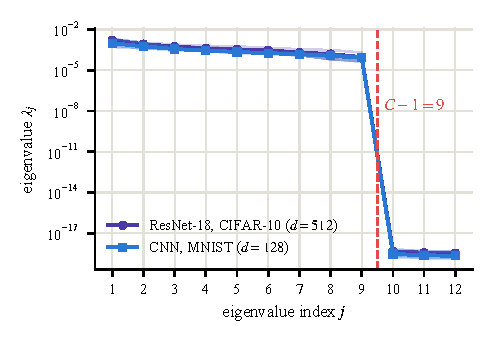
\includegraphics[width=0.9\columnwidth]{figures/fisher_spectrum}
\caption{Top twelve eigenvalues of the activation-space Fisher matrix, five
seeds per model (thin lines) and their mean (markers). Both 10-class models
show exactly $C-1=9$ informative eigenvalues followed by a drop of about
fourteen orders of magnitude, as the rank bound \eqref{eq:rank} predicts.}
\label{fig:spectrum}
\end{figure}

\subsection{Blind-Subspace Shift Tracks Measured Harm}
\label{sec:saturation}

On Rotated MNIST accuracy falls from 99\% to 13\% as the angle grows, and the
FEATHER score rises monotonically with it. On CIFAR-10-C (Fig.~\ref{fig:cifar})
the blind-shift score tracks the measured accuracy drop. At the episode level
these benchmarks do not separate the detectors: FEATHER, the covariance
ablation, and the confidence and entropy baselines all separate harmful from
benign at AUROC $1.0$ on both benchmarks and every seed. Corruption suites
produce \emph{output-visible} drift; what separates the monitors is how often
they alarm on drift that does no harm (Section~\ref{sec:alarms}).

\begin{figure}[t]
\centering
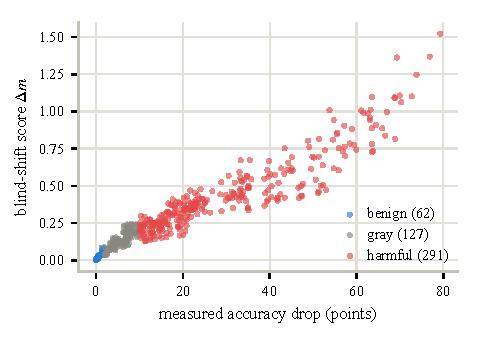
\includegraphics[width=0.9\columnwidth]{figures/results_cifar10c}
\caption{CIFAR-10-C, all 96 episodes and five seeds (480 points). The
blind-shift score grows with the measured accuracy drop.}
\label{fig:cifar}
\end{figure}

\subsection{Deep-Feature Silent Drift}
\label{sec:blinddeep}

The benchmarks never reach drift the outputs \emph{cannot} express. We
construct it on the trained ResNet-18's saved activations: onto a clean batch
we add a shift $\alpha u$ along a unit direction $u$ from $\mathcal{N}$ or from
$\mathcal{S}$. To measure harm, the ground-truth label depends on the sample's
coordinate along $u$, which the frozen head discards, and flips once a shifted
sample leaves its clean range; the correct label changes while every logit
stays fixed.

The contrast is unambiguous (Table~\ref{tab:blinddeep}, five seeds,
$\alpha=0.3$). A blind-subspace shift that triggers FEATHER on every batch
moves the most-changed softmax probability by under $2\times10^{-10}$, and mean
confidence and entropy by under $10^{-12}$, yet pushes the synthetic accuracy
from $99\%$ down to $7\%$. Under the sensitive-subspace control the outputs
move and FEATHER stays at its $2\%$ floor. The plain mean shift, at the same
budget, detects only $41\%$ of blind-drift batches at $\alpha=0.3$, and $5\%$
at $\alpha=0.2$, where accuracy has already fallen to $43\%$: clean-batch noise
in $\Delta\mu$ concentrates in the high-variance sensitive directions, which
FEATHER projects out, lowering its threshold by a factor of about $3.4$ ($0.11$
vs.\ $0.37$). Fig.~\ref{fig:blinddeep} follows these effects as $\alpha$
grows. Against the real labels of these reference images, accuracy stays at
$99.97\%$ in both directions: a shift that leaves every output unchanged cannot
change correctness against fixed labels, so the harm here exists only under the
synthetic rule. The experiment establishes output-invisibility and FEATHER
detection on a real network, not harm on natural data.

\begin{table}[t]
\caption{Deep-feature silent drift on the CIFAR-10 ResNet-18 at $\alpha=0.3$
(mean over five seeds). The synthetic rule reads only the blind coordinate, so
a sensitive shift cannot trigger it (--).}
\label{tab:blinddeep}
\centering
\footnotesize
\setlength{\tabcolsep}{3pt}
\begin{tabular}{lccccc}
\hline
Shift & Max output & FEATHER & Mean-shift & Real-label & Synthetic \\
direction & change & alarm & alarm & acc. & acc. \\
\hline
Blind ($\mathcal{N}$) & $1.7\times10^{-10}$ & $\mathbf{1.00}$ & $0.41$ & $1.00$ & $0.07$ \\
Sensitive ($\mathcal{S}$) & $6.3\times10^{-2}$ & $0.02$ & $0.46$ & $1.00$ & -- \\
\hline
\end{tabular}
\end{table}

\begin{figure}[t]
\centering
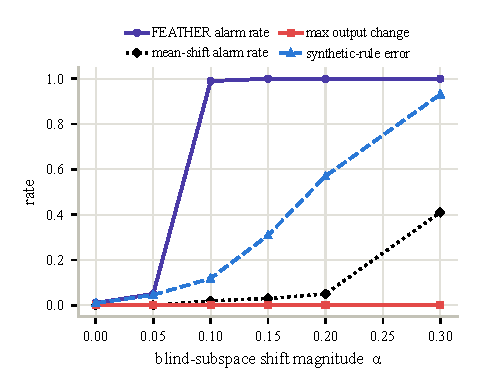
\includegraphics[width=0.9\columnwidth]{figures/blind_deep}
\caption{Blind-subspace drift on the trained ResNet-18. As the shift grows,
FEATHER alarms and the synthetic error climb together, while the largest change
in any model output stays on its $10^{-10}$ floor and the full-space mean
shift responds only once most of the damage is done.}
\label{fig:blinddeep}
\end{figure}

\subsection{Where the False Alarms Land}
\label{sec:alarms}

Table~\ref{tab:alarms} sets all seven monitors against the same CIFAR-10-C
episodes. The output baselines are calibrated on a held-out split of the clean
deployment stream; without that they alarm on every clean test batch, owing to
the train-to-test confidence gap. Because this drift is output-visible, the
output baselines perform best here ($6$--$9\%$ benign alarms), as
Proposition~\ref{prop:blind} predicts. FEATHER alarms more often
($47.6 \pm 6.9\%$), since a benign corruption can move the blind subspace while
sparing accuracy; a three-consecutive-batch run rule lowers this only to
$0.32 \pm 0.07$ (the output baselines' to at most $0.01$). Against its own
covariance ablation, however, FEATHER is clearly superior: the ablation alarms
on $82.9 \pm 6.9\%$ of benign batches, a gap of $35.3 \pm 3.6$ points that
stays positive on every seed (an exact paired sign-flip test over seeds gives
$p = 0.0625$, the smallest possible with five seeds). At the episode level the
gap is $34.4$ points (95\% bootstrap confidence interval $[27.9, 41.1]$), and a
paired sign-flip test over the 62 benign episodes gives $p < 10^{-4}$; the
ablation alarms more often than FEATHER in $77\%$ of benign episodes and less
often in none. Low-variance directions
move under benign corruption and even clean resampling (the ablation's $28\%$
clean rate); low-Fisher directions do not. The full-space mean shift alarms on
fewer benign batches than FEATHER ($0.20 \pm 0.03$, lower on every seed), but
its larger threshold makes it miss blind drift (Section~\ref{sec:blinddeep}).
At matched calibration, recalibrating FEATHER on a held-out split of the clean
\emph{test} stream keeps its clean false-alarm rate at $0.10 \pm 0.06$ on
CIFAR-10-C and $0.08 \pm 0.04$ on MNIST, and it still alarms on fewer benign
shifts than the ablation ($0.59 \pm 0.05$ vs.\ $0.67 \pm 0.05$) while both
detect every harmful one.

\textit{Detection delay.} We measure delay as the number of batches from the
first shifted batch to the first alarm. Every monitor alarms on the first
batch of every harmful episode. On gray episodes FEATHER and the covariance
ablation again alarm on the first batch, while the output baselines need
$1.17$--$1.47$ batches on average and up to ten in the worst case.

\begin{table}[t]
\caption{Batch-level alarm rates on CIFAR-10-C (mean over five seeds). Output
baselines are calibrated on half of the clean test stream and scored on the
other half; the other monitors on the training reference.}
\label{tab:alarms}
\centering
\footnotesize
\begin{tabular}{lcccc}
\hline
Monitor & Clean & Benign & Gray & Harmful \\
\hline
ATC \cite{garg2022atc} & $0.00$ & $\mathbf{0.06}$ & $0.82$ & $1.00$ \\
Confidence drop & $0.00$ & $0.07$ & $0.89$ & $1.00$ \\
Entropy rise & $0.00$ & $0.09$ & $0.93$ & $1.00$ \\
Error proxy \cite{amoukou2024sequential} & $0.00$ & $\mathbf{0.06}$ & $0.88$ & $1.00$ \\
\hline
Mean shift $\lVert\Delta\mu_t\rVert$ & $0.00$ & $0.20$ & $0.94$ & $1.00$ \\
Covariance ablation & $0.28$ & $0.83$ & $1.00$ & $1.00$ \\
FEATHER & $0.02$ & $0.48$ & $1.00$ & $1.00$ \\
\hline
\end{tabular}
\end{table}

\subsection{Ablation Study}
\label{sec:ablation}

FEATHER combines three components: a subspace chosen by the Fisher spectrum,
the restriction of the shift statistic to that subspace, and calibration on
held-out data. Table~\ref{tab:ablation} removes the first two one at a time
and reports each variant on clean and benign CIFAR-10-C batches and on the
silent-drift experiment of Section~\ref{sec:blinddeep} ($\alpha=0.3$, blind
shift and sensitive control). Replacing the Fisher subspace by the
covariance subspace of the same dimension keeps the detection of blind drift
but loses selectivity: the variant alarms on $28\%$ of clean, $83\%$ of benign,
and $89\%$ of sensitive-control batches, the last being drift the output
monitors already see. Removing the subspace restriction, i.e.\ using the
full-space mean shift, lowers benign alarms to $20\%$ but detects only $41\%$
of blind-drift batches, because clean-batch noise in the sensitive directions
raises its threshold. Only the Fisher subspace both detects blind drift and
stays silent on output-visible drift. Removing held-out calibration, i.e.\
setting thresholds on the training reference when it does not match the
deployment stream, makes FEATHER alarm on every clean MNIST test batch;
calibrated on held-out clean test data, its rate falls to $8\%$.

\begin{table}[t]
\caption{Ablation of FEATHER's components (mean alarm rates over five seeds).
Clean and benign: CIFAR-10-C batches. Blind and sensitive: silent-drift
experiment at $\alpha=0.3$ (Section~\ref{sec:blinddeep}).}
\label{tab:ablation}
\centering
\footnotesize
\setlength{\tabcolsep}{4pt}
\begin{tabular}{lcccc}
\hline
Variant & Clean & Benign & Blind & Sensitive \\
\hline
FEATHER (Fisher subspace) & $0.02$ & $0.48$ & $\mathbf{1.00}$ & $\mathbf{0.02}$ \\
Covariance subspace & $0.28$ & $0.83$ & $1.00$ & $0.89$ \\
Full space (mean shift) & $0.00$ & $0.20$ & $0.41$ & $0.46$ \\
\hline
\end{tabular}
\end{table}

\subsection{Natural Shift on Real Data}
\label{sec:wilds}

\textit{Hospital shift.} We use WILDS Camelyon17 \cite{koh2021wilds}, a binary
tumour-vs-normal patch task whose domains are hospitals. A ResNet-18 trained on
the in-distribution hospitals ($98.8\%$ validation accuracy) is monitored as
the two held-out hospitals stream in. As the rank bound predicts for a binary
task, one Fisher eigenvalue ($1.5\times10^{-2}$) sits above a cliff to
$\sim10^{-18}$, leaving $511$ of $512$ dimensions blind. Accuracy falls from
$99.0\%$ in distribution to $69.5\%$ and $58.5\%$ on the two out-of-domain
hospitals, and FEATHER tracks it, staying within its budget in distribution
and alarming on every batch of both shifted hospitals. The output baselines
alarm on all shifted batches too: stain and morphology changes are
output-visible.

\textit{Subpopulation shift.} Harm with unchanged outputs requires new inputs
with their own labels, so we pre-registered a BREEDS-style shift
\cite{santurkar2021breeds}: a ResNet-18 trained on the 20 CIFAR-100
superclasses using four of the five subclasses of each ($83.0 \pm 0.8\%$
accuracy) monitors streams in which a fraction $\rho$ of each batch comes from
the held-out subclasses. The pre-registered criterion, a drop of at least ten
points flagged by FEATHER while every output baseline stays below $20\%$
alarms, was not met. The output baselines, calibrated as in
Section~\ref{sec:alarms}, reach $50\%$ alarms at $\rho = 0.2$ (a $7.8$-point
drop); FEATHER, calibrated on the training reference ($7\%$ clean false
alarms), at $\rho = 0.3$ ($12.0$ points); the mean shift only at $\rho = 0.8$.
Across 20 single-superclass swaps the drop correlates with the output scores
(Spearman $0.85$--$0.87$) and negatively with FEATHER's blind fraction $s$
($-0.86$): harmful subclasses shift mainly along the sensitive directions. This
shift, too, is output-visible.

\subsection{Cost and a Two-Stage Cascade}
\label{sec:cascade}

For the ResNet-18 the offline fit, including the forward passes over
50{,}000 images, takes 11.1 s; online, FEATHER's statistics take 3.0 ms per
500-image batch on a laptop CPU, small next to the forward pass. The output
baselines cost only a reduction over softmax outputs the model already
produces. Since FEATHER's statistic is the blind part of
$\lVert\Delta\mu\rVert$, the full-space shift (0.05 ms) serves as a gate, and
the projection runs only when it alarms. On CIFAR-10-C the cascade matches
FEATHER-always on harmful episodes ($0.80$ vs.\ $0.82$ of batches) and alarms
on $16\%$ of benign batches against $40\%$; on Rotated MNIST the gate fires on
almost every batch, so it saves nothing.

\section{Discussion and Limitations}
\label{sec:limitations}

On corruption suites, whose drift is output-visible, FEATHER does not beat the
output monitors on false alarms; in the silent regime of
Section~\ref{sec:blinddeep} it is the only effective one. The two are
complementary: a confidence monitor for visible failures, FEATHER for blind
ones. Choosing the subspace by the Fisher spectrum rather than by variance
nearly halves the covariance ablation's benign alarms, since the discarded
low-Fisher directions are those the decisions ignore.

Pure concept shift that leaves the activation marginals alone is invisible to
every label-free method, ours included. The silent-regime result is
semi-synthetic (drift injected in activation space, harm from a synthetic
rule), and both natural shifts we tested are output-visible; a natural shift
that brings in differently labelled inputs whose outputs match the reference
remains the most valuable next step. Held-out calibration holds the clean
false-alarm rate at budget only when the reference data matches the deployment
stream: calibrated on its training split, FEATHER alarms on every clean MNIST
test batch, and on $8\%$ once recalibrated on clean test data.

Mixed drift, which moves the activations along sensitive and blind
directions at once, is split by construction: FEATHER responds only to the
blind component, and the direction ratio $s_t$ reports what fraction of the
shift it accounts for, while the sensitive component is left to the output
monitors. A deployment should therefore run both; we have not evaluated
streams in which the two components change at different times. For
high-dimensional models the cost grows linearly in $d$
(Section~\ref{sec:complexity}), but the blind subspace then covers an even
larger share of the representation, so the bootstrap thresholds need enough
clean reference batches to estimate the noise of a high-dimensional
projection. Finally, the blind subspace belongs to the penultimate layer; a
Kronecker-factored approximation of the Fisher matrix would extend it to
intermediate layers.

\section{Conclusion}
\label{sec:conclusion}

The geometry of a softmax head makes the price of output-based monitoring
exact: the outputs are a $(C-1)$-dimensional window onto a $d$-dimensional
representation, and everything orthogonal to it is invisible. FEATHER computes
the invisible part exactly and monitors it at the cost of a single projection.
It follows measured harm, nearly halves the false alarms of its covariance
ablation, and, in the semi-synthetic setting, is the only monitor that detects
harmful drift the outputs cannot express, complementing confidence-based tools
in the one region they provably cannot reach.

\section*{Acknowledgment}
The authors thank the School of Technology Management and Engineering
(STME), SVKM's NMIMS, Indore for providing computational and GPU facilities
to conduct this research. This research received no external grant funding.

\bibliographystyle{IEEEtran}
\bibliography{References}

\end{document}
